\documentclass{standalone}
\usepackage{pgfplots}
\usepgfplotslibrary{fillbetween}
\usetikzlibrary{patterns.meta}
\pgfplotsset{compat=1.18}
\renewcommand{\familydefault}{\sfdefault}

\begin{document}
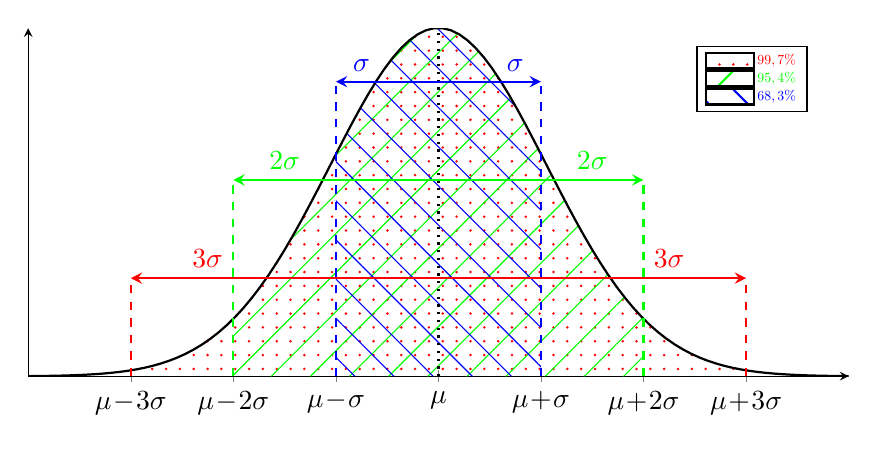
\begin{tikzpicture}
\begin{axis}[
    legend style = {
        at={(0.95,0.95)}, 
        anchor=north east,
        cells={anchor=west}
    },
    axis lines = left,
    samples=100,
    domain=40:160,
    xtick={55, 70, 85, 100, 115, 130, 145},
    scaled ticks=false,
    xticklabels={
        $\mu{\!}-{\!}3\sigma$,
        $\mu{\!}-{\!}2\sigma$, 
        $\mu{\!}-{\!}\sigma$, 
        $\mu$, 
        $\mu{\!}+{\!}\sigma$, 
        $\mu{\!}+{\!}2\sigma$,
        $\mu{\!}+{\!}3\sigma$
    },
    ytick=\empty,
    yticklabels={},
    height=6cm,
    width=12cm,
    no markers,
    every axis plot/.append style={thick},
    legend style = {
        nodes={scale=0.5}
    }
]   
    % Gaußkurve
    \addplot [black, name path=gauss, forget plot] 
        {1/(15*sqrt(2*pi)) * exp(-((x-100)^2)/(500))};

    % Vertikale Linien und Pfeile
    \draw [black, thick, dotted] (axis cs:100, 0) -- (axis cs:100,0.3);
    \pgfplotsinvokeforeach{55,145}{
        \draw [red, thick, dashed] (axis cs:#1, 0) -- (axis cs:#1,0.0075);
        \draw [red, thick, -stealth] (axis cs: 100,0.0075) 
            -- node[above, near end] {$3\sigma$}
            (axis cs:#1,0.0075);
    }
    \pgfplotsinvokeforeach{70,130}{
        \draw [green, thick, dashed] (axis cs:#1, 0) -- (axis cs:#1,0.015);
         \draw [green, thick, -stealth] (axis cs: 100,0.015) 
            -- node[above, near end] {$2\sigma$}
            (axis cs:#1,0.015);
    }
    \pgfplotsinvokeforeach{85,115}{
        \draw [blue, thick, dashed] (axis cs:#1, 0) -- (axis cs:#1,0.0225);
        \draw [blue, thick, -stealth] (axis cs: 100,0.0225) 
            -- node[above, near end] {$\sigma$}
            (axis cs:#1,0.0225);
    }

    % Unsichtbarer Pfad auf x-Achse für Flächenberechnung
    \path[name path=axis] (axis cs:40,0) -- (axis cs:160,0);

    % Flächen
    \addplot [
        pattern={Dots[distance=5pt]}, 
        pattern color=red,
        area legend
        ] 
        fill between[
        of=gauss and axis, 
        soft clip={domain=55:145}
        ];
        \addlegendentry{\color{red} $99,7\%$}
    \addplot [pattern={Lines[angle=45, distance=10pt]}, 
    pattern color=green,
    area legend
    ] 
    fill between[
        of=gauss and axis, 
        soft clip={domain=70:130}
        ];
    \addlegendentry{\color{green} $95,4\%$}
    \addplot [pattern={Lines[angle=135, distance=10pt]}, 
    pattern color=blue,
    area legend] 
    fill between[
        of=gauss and axis, 
        soft clip={domain=85:115}
        ];
    \addlegendentry{\color{blue} $68,3\%$}
    



    
\end{axis}
\end{tikzpicture}
\end{document}
